\documentclass[12pt]{article}
\usepackage[utf8]{inputenc}
\usepackage{amsmath}
\usepackage{mathtools}
\usepackage{amsfonts}
\usepackage{lastpage}
\usepackage{tikz}
\usepackage{pdfpages}
\usepackage{gauss}
\usepackage{fancyvrb}
\usepackage{fancyhdr}
\usepackage{graphicx}
\pagestyle{fancy}
\fancyfoot[C]{\footnotesize Page \thepage\ of 5}
\DeclareGraphicsExtensions{.pdf,.png,.jpg}
\title{Lynopgave 1}
\author{Nikolaj Dybdahl Rathcke and Victor Petren Bach Hansen}
\chead{Nikolaj Dybdahl Rathcke (rfq695) - Victor Petren Bach Hansen (grn762)}

\begin{document}
\section*{MatIntroNat - Lynopgave 2}
\subsection*{4.1}
Løs differentialligningen
$$(1+x^2)yy\prime=x(1+y^2)$$
med hver a begyndelsesbetingelserne
$$y(3)=1,\:y(3)=3,\:y(3)=-7$$
Opgaven skal først løses med Maple, dernæst uden ved separation.\\
\\
Differentiligningen defineres i Maple\\
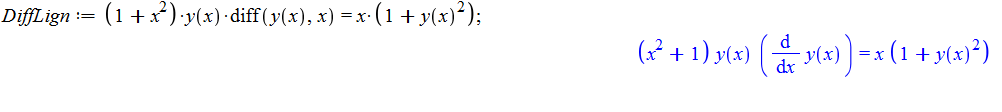
\includegraphics[scale=0.6]{41a1}\\
Herefter løses den med de 3 forskellige begyndelsesværdier.\\
For $y(3)=1$\\
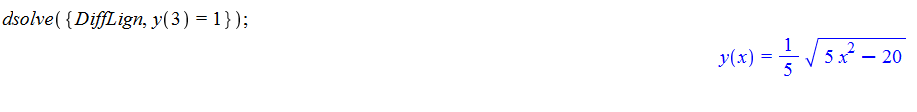
\includegraphics[scale=0.6]{41a2}\\
For $y(3)=3$\\
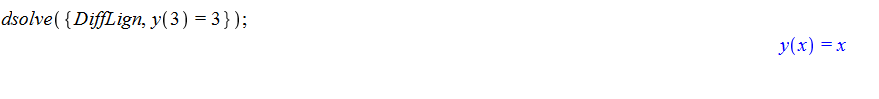
\includegraphics[scale=0.6]{41a3}\\
For $y(3)=-7$\\
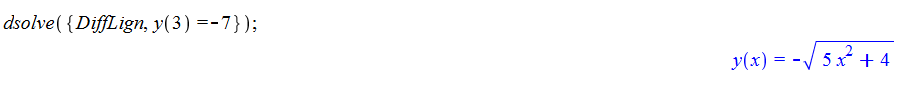
\includegraphics[scale=0.6]{41a4}\\
Dernæst løses det uden brug af Maple på følgende måde
$$(1+x^2)yy\prime=x(1+y^2)\Leftrightarrow$$
$$\dfrac{yy\prime}{(1+y^2)}=\dfrac{x}{1+x^2} \Leftrightarrow$$
$$\int \dfrac{y}{1+y^2}\dfrac{dy}{dx} dx = \int \dfrac{x}{1+x^2} dx \Leftrightarrow$$
$$\int \dfrac{1}{1+y^2} y \: dy = \int \dfrac{1}{1+x^2}x\: dx \Leftrightarrow$$
Vi går nu over til at regne på venstreside, da vi har to 'ens' udtryk på begge sider med forskellig variabel.\\
$u$ bliver nu substitueret ind:
$$u=1+y^2 \Rightarrow$$
$$\dfrac{du}{dy}=2y \Leftrightarrow y = \dfrac{1}{2} \dfrac{du}{dy}$$
Vi indsætter nu denne $y$ værdi i udtrykket
$$\int \dfrac{1}{1+y^2} y \: dy$$
og får følgende
$$\int \dfrac{1}{2} \dfrac{du}{dy} \dfrac{1}{u}\: dy = \int \dfrac{1}{2}\dfrac{1}{u}\: du = \dfrac{1}{2} \int \dfrac{1}{u} \: du = \dfrac{1}{2}\ln(|u|)$$
Da vi som før nævnt at vi på begge sider havde to samme udtryk med forskellig varibel, benyttes samme fremgangmåde som ovenfor til at komme frem til (hvor $u$ er substitueret tilbage til $1+y^2$ og $1+x^2$).\\ 
Det observeres ligeledet at da $y^2$ og $x^2$ altid vil være to positive tal for alle reelle tal, fjernes absolut-tegnene:
$$\int \dfrac{1}{1+y^2} y \: dy = \int \dfrac{1}{1+x^2}x\: dx \Leftrightarrow$$
$$\dfrac{1}{2}\ln(1+y^2) =\dfrac{1}{2}\ln(1+x^2) + C$$
$$e^{\ln(1+y^2)} = e^{\ln(1+x^2)+C} \Leftrightarrow$$
$$1+y^2=e^{C}(1+x^2) \Leftrightarrow$$
$$1+y^2=C(1+x^2)\Leftrightarrow$$
$$y^2=C(1+x^2)-1\Leftrightarrow$$
$$y=\pm \sqrt{C(1+x^2)-1}$$
Vha. denne generelle formel vil vi nu finde $y(x)$ med de $3$ forskellige begyndelsesværdier.\\
Først for $y(3)=1$:
$$1=\sqrt{C(1+3^2)-1} \Leftrightarrow 1^2 = 10C-1 \Leftrightarrow 2=10C \Leftrightarrow C = \dfrac{1}{5}$$
Dernæst for $y(3)=3$
$$3=\sqrt{C(1+3^2)-1}\Leftrightarrow 3^2 = 10C-1 \Leftrightarrow 10=10C \Leftrightarrow C= 1$$
Og til sidst for $y(3)=-7$
$$-7=\sqrt{C(1+3^2)-1}\Leftrightarrow -7^2 = 10C-1 \Leftrightarrow 50=10C \Leftrightarrow C= 5$$
Og således er de 3 forskellige $C$ værdier fundet.
\newpage
\subsection*{4.2(i)}
(a) løses uden Maple, (b) og (c) løses med Maple

\subsubsection*{a}
Find den fuldstændige løsning til differentialligningen
$$y\prime\prime+2y\prime-3y=0$$
\\
Vi finder rødderne til ligningen $r^2+2r-3=0$
$$r_1=\frac{-b+\sqrt{b^2-4ac}}{2a}=\frac{-2+\sqrt{2^2-4*1*(-3)}}{2*1}=\frac{2}{2}=1$$
$$r_2=\frac{-b-\sqrt{b^2-4ac}}{2a}=\frac{-2-\sqrt{2^2-4*1*(-3)}}{2*1}=\frac{-6}{2}=-3$$
Da den har rødderne $1,-3$ har den homogene ligning, af sætning 10.5.3 i TL, den fuldstændige løsning
$$y(x)=c_1e^{r_1x}+c_2e^{r_2x}=c_1e^{x}+c_2e^{-3x}$$

\subsubsection*{b}
Find for enhver reel værdi af konstanten $a$ den fuldstændige løsning til differentialligningen
$$y\prime\prime+2y\prime-3y=e^{ax}$$
\\
Nedenfor er differentialligning defineret og løst i Maple:\\
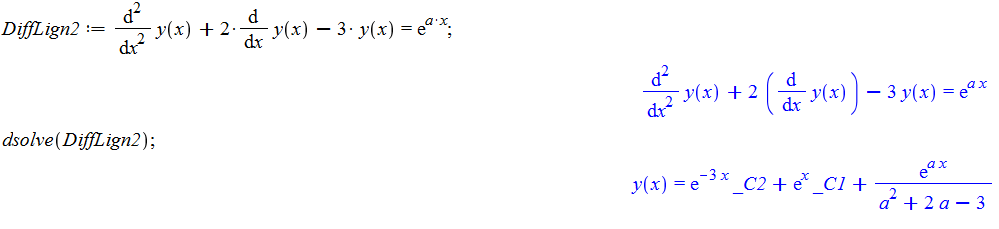
\includegraphics[scale=0.6]{42b1}
Hvilket er den fuldstændige løsning til differentialligning hvor $\_C2$ og $\_C1$ er konstanter.

\subsubsection*{c}
Find, stadig for alle $a$, den partikulære løsning $y(x)$ til problemet i (b) som opfylder $y(0)=y\prime(0)=0$\\
\\
Herunder ses, beregnet med Maple, den partikulære løsning\\
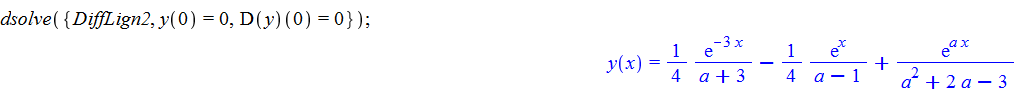
\includegraphics[scale=0.6]{42c1}\\
der opfylder $y(0)=y\prime(0)=0$.

\end{document}



